\chapter{Amplifier Classes}
The generic power amplifier consists of a transistor with a DC bias and AC coupled to the RF input and output ports. For the sake of simplicity this paper will describe the operation of FET amplifiers. The major source of power consumption of an amplifier comes from the drain source current that flows during operation. By reducing the current flow, the power added efficiency (PAE) of the amplifiers can be increased
Power amplifiers come in a variety of classes, and the most commonly used ones are A, B, AB, C, D, E, and F. Classes A through C can be described by the conduction angle of the device. The conduction angle is the amount of current flowing through the transistor from drain to source during a single cycle of the AC signal being amplified ranging from 0 to 2$\pi$ \cite{Colantonio1998}. Classes D through F are defined as switching amplifiers and vary due to the output matching network which shape the waveforms of the current and voltage at the drain of the device.

For class A, the conduction angle is 2$\pi$ meaning current is always flowing when the amplifier is on increasing the power consumption. Class A does have the advantage of having the highest gain at a given frequency compared to other classes and also can operate near the frequency limit of a transistor .\cite{} Class A also has the highest linearity, lowest harmonic distortion, and is advantageous when high dynamic range is required .\cite{C.Cripps2006} Class B has a conduction angle of $\pi$ so current only flows during half the cycle of the AC signal reducing power consumption. Class AB has a conduction angle between $\pi$ and 2$\pi$. Class E is a type of harmonic termination that uses capacitive terminations at the output to achieve 100\% efficiency.

% Citations are wrong above!

\section{Efficiency of Amplifiers}

To reduce the power consumption of a power amplifiers, two major concepts are important: zero voltage switching (ZVS) and zero voltage derivative switching (ZVDS). ZVS is when as the name implies, there is zero voltage when the amplifier is switched on and conducting so while current flows through the output no power is consumed. ZVDS is when there is no overlap between the voltage and current waveforms so no power is consumed during switching. If an amplifier can achieve ZVS and ZVDS it would theoretically be 100\% efficient. A measure of amplifier efficiency is the power added efficiency (PAE) defined in equation~\ref{pae}. PAE is a measure of how efficient an amplifier is able to convert the input DC power into RF power gain. Ideally all of the DC power used to power the amplifier would be used to increase the input RF power. The maximum limit for a lossless system is 100\%, for example if a power amplifier consumed 1 Watt and was able to output 1.001 Watt of RF power from 1 mW of RF input power, the PAE would be 100.\% because all of the DC power was used to increase the RF power.

\begin{equation}\label{pae}
  PAE,\% = \frac{RF Power_{out} - RF Power_{in}}{DC Power}
\end{equation}

\section{Class A Amplifier}

The class A amplifier uses a bias that results in a conduction angle of 2$\pi$ which results in power always being consumed due to the constant bias current and voltage present at the drain of the amplifier. The bias point is chosen so the transistor operates in the active region which can be seen in Figure \ref{classa_bias}. The constant power consumption limits the maximum efficiency of the class A amplifier to 50\% \cite{C.Cripps2006}. 
The class A amplifier is the most linear of all classes due to the conduction angle. The high linearity allows the class A amplifier to have the lowest intermodulation distortion (IMD) of all the amplifier classes. The downside of the linearity is that the input drive level is proportional to the IMD present at the output of the amplifier. Class A amplifiers are also able to operate closer to the highest operating frequency of a transistor due to lack of harmonics used in the amplifier \cite{}. %ham paper

The class A amplifier is similar to the small signal amplifier in many ways.

%Fix all the citations lol

\begin{figure}
  \centering
  % Requires \usepackage{graphicx}
  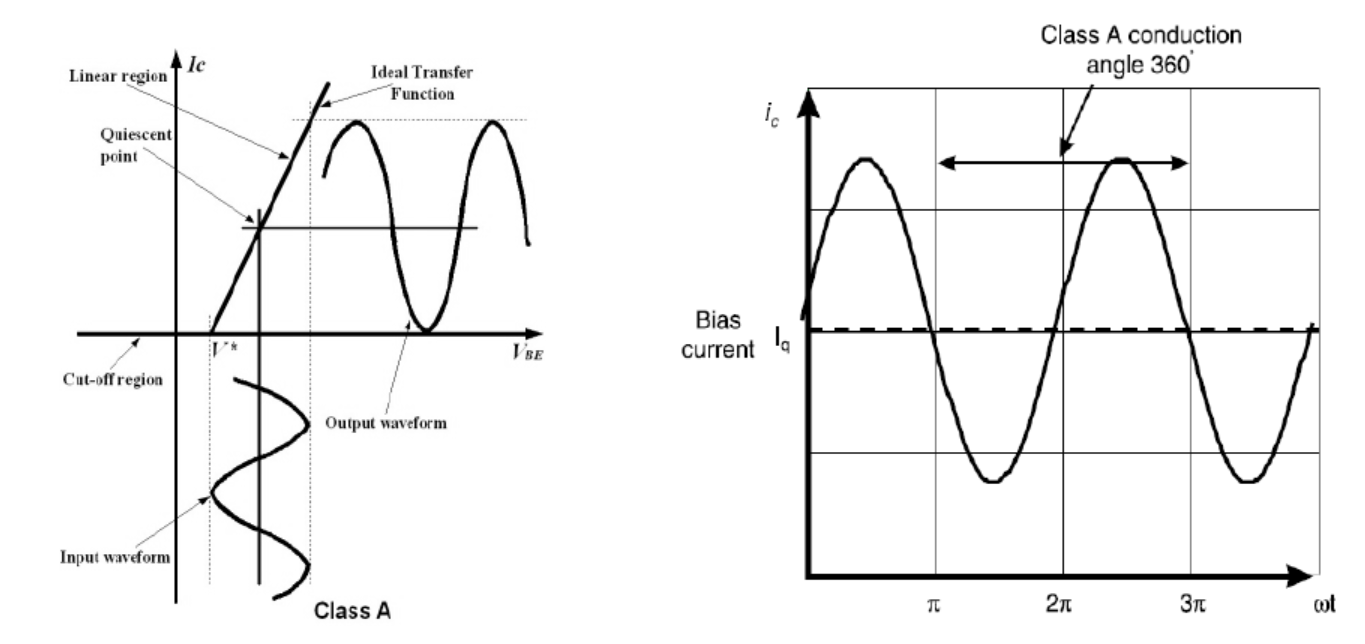
\includegraphics[width=6in]{figures/classa}
  \caption{Class A Bias Point and Conduction Cycle}\label{classa_bias}
\end{figure}

\section{Class B Amplifier}

* Conduction angle of $\pi$
* 

Class B uses a conduction angle of $\pi$.

\section{Class AB Amplifier}

\section{Class C Amplifier}

\section{Class D Amplifier}

\section{Class E Amplifier}



\section{Class F Amplifier}

The class F amplifier has a theoretical efficiency of 100\% through the use of multi harmonic terminations. The theory behind the class F amplifier relies on the generation of odd voltage harmonics and shorting of even voltage harmonics at the drain of the device to increase the efficiency of the amplifier. By keeping only the odd harmonics of the signal at the output, ideally a square wave would appear and by biasing the amplifier at a conduction angle of pi the amplifier has zero overlap between the current and voltage waveforms and no power consumed when the amplifier is switched on.
The harmonics are generated due to the knee voltage of the transistor. When the AC signal causes the transistor to reach saturation the abrupt change in current flow generates voltage harmonics. In practice it becomes challenging to design matching networks as the number of harmonics to control increases. Also the output capacitance of the transistor will eventually short out higher order harmonics so 100\% efficiency is not realizable in practice. By controlling up to the 5th harmonic, 90.5\% efficiency can be achieved.

